\section{Sampling scheme}
\label{sec:sampl_scheme}
There are many different ways to sample a sphere \cite{Zhang2012575}, as also discussed in Section \ref{sec:rel_res:sampl_sch}.
The turntable can be controlled with \matlab, the elevation of the loudspeaker on the arc however has to be adjusted by hand. Therefore, sampling schemes with as few manual operations as possible will be considered.
Replacing the loudspeaker is very time consuming and therefore undesirable.

To minimize the error margins, a maximum distance between two sampling points of half the minimum wavelength of the desired signal is taken into account.
A speed of sound of $v_\text{air}=344$ m/s is considered and the maximum frequency in a human voice is around $f_{\text{voice}_\text{max}}=8$ kHz \cite{hospital}, although for most applications in communication and speech enhancement a maximum of just 3.5 kHz is taken into account \cite[p.~58]{book:jorge_speechenhancement}.
Because the objective of this project concerns application in speech, frequencies above 8 kHz are of less value.
This gives a maximum distance between two sampling points of 2.15 cm \eqref{eqn:ontwerp_afstandmin}.

The sphere which will be sampled, is the sphere with centre the microphone of the smartphone and radius the length of the smartphone.
Within this sphere the behaviour of the sound is influenced by the smartphone and outside this sphere not, so the choice for the smallest sphere is made.
The smartphone has a length of $\ell_\text{phone}=13.87$ cm. The length of the equator of the sphere is $\ell_\text{eq}=2\pi\ell_\text{phone}\approx87.1$ cm.

There are two sampling schemes taken in account, which both feature a low number of movements about the $\phi$-direction, which shortens the execution time of the experiment,

\begin{equation}
\label{eqn:ontwerp_afstandmin}
\Delta\ell_\text{max}=\dfrac{\lambda_\text{min}}{2}=\dfrac{1}{2}\dfrac{v_\text{air}}{f_{\text{voice}_\text{max}}}=\dfrac{344}{16000}=2.15\text{ cm}.
\end{equation}

\subsection{Equiangular}
\label{ssec:equiangular}
An equiangular sampling scheme has equal angles between two neighbouring samples, so the sphere is divided into longitudes and latitudes.
In the direction of $\theta$ samples will be taken over $360^\circ$ and in the $\phi$-direction over $180^\circ$.
It is therefore important that the difference in angle between two sampling points is a common divisor of 180 and 360.
The distance around the equator is the circle with the largest distance between two sampling points on the sphere. 
On the equator the maximum distance between two sampling points thus is\footnote{For small angles the distance over the sphere is approximately the same as the direct distance, therefore this equation will be used.} 
\begin{equation*}
\Delta\ell_\text{max}\geq\ell_\text{eq}\cdot\dfrac{360^\circ}{\Delta\theta}.
\end{equation*}
The largest common divisor smaller than 8.9 is 7.5.
This yields 24 longitudes and 48 latitudes, for a total of $23\cdot 48+2=1106$ sampling points (when taken into account that on the poles there is only one sampling point).

In practice this cannot be done, because the turntable only turns in full degrees.
The first common divisor smaller than 8.9 is 6, this gives 30 longitudes and 60 latitudes, so a total of $29\cdot60+2=1742$ sampling points.
It would be more comprehensive to choose angles of $9^\circ$, which lowers the largest frequency, but it is more practical because it results in $19\cdot 40+2=762$ sampling points.

\subsection{IGLOO}
The other sampling scheme taken into account is the IGLOO sampling scheme \cite{Zhang2012575}.
The IGLOO sampling scheme divides the surface of the sphere in 12 faces, from now on called base faces, of approximately the same surface area.
The following base faces are used:
\begin{multicols}{2}
\begin{itemize}
\item[]\textbf{North pole}
\item $\phi\in[0^\circ,60^\circ]$, $\theta\in[0^\circ,120^\circ]$
\item $\phi\in[0^\circ,60^\circ]$, $\theta\in[120^\circ,240^\circ]$
\item $\phi\in[0^\circ,60^\circ]$, $\theta\in[240^\circ,360^\circ]$
\item[]\textbf{Middle}
\item $\phi\in[60^\circ,120^\circ]$, $\theta\in[0^\circ,60^\circ]$
\item $\phi\in[60^\circ,120^\circ]$, $\theta\in[60^\circ,120^\circ]$
\item $\phi\in[60^\circ,120^\circ]$, $\theta\in[120^\circ,180^\circ]$
\item $\phi\in[60^\circ,120^\circ]$, $\theta\in[180^\circ,240^\circ]$
\item $\phi\in[60^\circ,120^\circ]$, $\theta\in[240^\circ,300^\circ]$
\item $\phi\in[60^\circ,120^\circ]$, $\theta\in[300^\circ,360^\circ]$
\item[]\textbf{South pole}
\item $\phi\in[120^\circ,180^\circ]$, $\theta\in[0^\circ,120^\circ]$
\item $\phi\in[120^\circ,180^\circ]$, $\theta\in[120^\circ,240^\circ]$
\item $\phi\in[120^\circ,180^\circ]$, $\theta\in[240^\circ,360^\circ]$.
\end{itemize}
\end{multicols}
A sphere, partitioned in this way, with 64 sampling points per base face is shown in Figure \ref{fig:IGLOO}.

Assuming the same minimal distance between two sampling points on the equator of $\Delta\ell$, the sphere will be divided with $\Delta\phi=7.5^\circ$, because $\phi\in[0^\circ,180^\circ]$ can be divided in three parts of $60^\circ$.
$\Delta\theta_\text{middle}=7.5^\circ$ in the middle, because this can also be divided in pieces of $60^\circ$.
This gives a total number of sampling points in the middle part of $s_\text{middle}=7\cdot48=336$.

For the pole faces the sampling is not equiangular like in the middle part.
The following is applicable to both the north as the south pole of the sphere.
The $\Delta\phi=7.5$ is the same as in the middle part.
Assume $\Delta\theta_\text{pole}$ \eqref{eq:delta_pole} and $\Delta\theta$ have to be a common divisor of 120.
$\ell_{60^\circ}=2\cdot(\cos(30^\circ)\cdot\ell_\text{phone})\cdot\pi=74.98$ cm.
It then follows that $\Delta\theta_\text{pole}\leq10.32^\circ$, so a $\Delta\theta_\text{pole}=10^\circ$ will be used,

\begin{equation}
\label{eq:delta_pole}\Delta\theta_\text{pole}\leq\dfrac{360^\circ\cdot\Delta\ell_\text{max}}{\ell_{60^\circ}}.
\end{equation}

The poles are divided in three faces of $120^\circ$. The sampling points have to be placed so they still meet the requirement of $\Delta\ell_\text{max}=2.15$ cm.
Per face this gives a distribution like can be found in Figure \ref{fig:poolvlak}.
This ideal case is by coincidence also the sphere given in Figure \ref{fig:IGLOO} (page \pageref{fig:IGLOO}).

\begin{wrapfigure}{r}{0.5\textwidth}
    \centering
    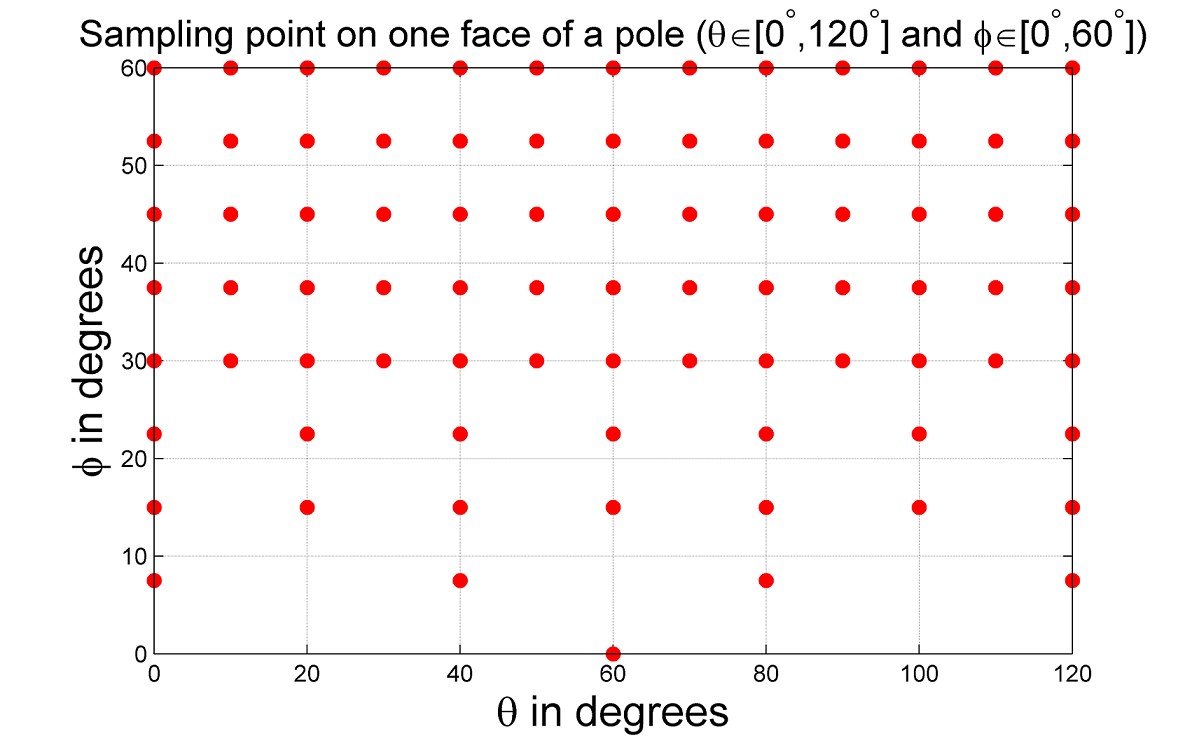
\includegraphics[width=0.5\textwidth]{afbeeldingen/poolvlak_optimaal.png}
    \caption{Distribution of sampling points on one face of the pole}
    \label{fig:poolvlak}
\end{wrapfigure}
This sampling scheme gives $s_\text{pole}=3\cdot(5\cdot12+2\cdot6+3)+1=226$ sampling points at the poles.
The full sampling scheme gives a total of 788 sampling points.
This theoretical case is not usable, because the turntable cannot turn half degrees. Because the middle of sphere has to be sampled equiangular, this gives $\Delta\theta_\text{middle}=\Delta\phi=6^\circ$ (9 is no divisor of 60), from which oversampling follows and this gives much more datapoints than the 762 of the equiangular method.

\subsection{Sampling scheme of choice}
The IGLOO sampling scheme seems appropriate for smaller angles (or larger spheres), because the requirements at $\Delta\theta$ of being a common divisor of 60 and 120 are easy applicable for those cases.
The sampling scheme used for the measurements is the equiangular scheme, because it has less sampling points than the IGLOO method and it is accurate for frequencies up to\footnote{If the assumption from the beginning of section \ref{sec:sampl_scheme} is followed.}
\begin{equation*}
f_\text{measure}=\dfrac{360\cdot v_\text{air}}{2\cdot\Delta\theta\cdot\ell_\text{eq}}=\dfrac{360\cdot344}{2\cdot9\cdot0.871}\approx7898\text{ Hz.}
\end{equation*} 

According to the method of Ajdler et al. \cite[eq.~(5)]{Ajdler2005III273}, the density of this sampling scheme should be accurate enough for frequencies up to 21.9 kHz \eqref{eq:ajdler}, which is higher than the maximum tone a human can hear (about 20 kHz).
\begin{equation}
\label{eq:ajdler}
\omega_t=\dfrac{cl_\theta}{0.137}=\dfrac{v_\text{sound}\cdot\Delta\theta}{0.137}=\dfrac{334\cdot 9}{0.137}\approx 21.9 \text{ kHz}
\end{equation}